\documentclass[11pt]{report}

\special{papersize=8.5in,11in}

\topmargin -0.5in \oddsidemargin 0.00in \evensidemargin 0.00in
\textwidth 6.75in \textheight 9.0in \headheight 0.25in \headsep
0.25in \footskip 0.5in \hoffset 0in \marginparpush 0.0in
\marginparwidth 0.0in \marginparsep 0.2in

\setcounter{page}{1}

\newcommand{\D}{\displaystyle}\newcommand{\T}{\textstyle}
\newcommand{\e}{{\mathrm{exp}}}
\newcommand{\dd}{{\mathrm d}}
\newcommand{\comment}[1]{}
\newcommand{\mb}{\mathbf}
\reversemarginpar

\usepackage[final]{graphicx}
\usepackage{fancyhdr}
%\graphicspath{{Papers/}}
\usepackage{amsthm,amssymb,amsmath}
\usepackage{cite}
\usepackage{geometry}
\usepackage{amsmath}
\usepackage{booktabs}
\usepackage{color}
\usepackage{setspace}
\usepackage{subfigure}
\usepackage{url}
%\usepackage{algorithm}
\usepackage{algorithmic}
\usepackage[ruled]{algorithm2e}
%\usepackage[top=2.5cm, bottom=2.5cm, right=3.5cm, left=3.5cm]{geometry}
\geometry{a4paper,scale=0.8}
\setcounter{secnumdepth}{3}

\title{Research Progress Report}

\author{Botao Zhu}

\begin{document}
	
	\maketitle
	\lhead{\sf Research Progress Report-7th} \chead{} \rhead{\sf Botao Zhu}
	\lfoot{CTRG, University of Saskatchewan} \cfoot{} \rfoot{Page \thepage}
	\renewcommand{\footrulewidth}{1.0pt}
	\renewcommand{\headrulewidth}{2.0pt}
	\renewcommand{\arraystretch}{1.3}
	\pagestyle{fancy}
	
	\renewcommand{\thesection}{\arabic{section}}
	
	\section{Reading and Research Activities}
	
	\subsection{Reading Summary}
	In order to prolong the life time of wireless network of LEACH protocol, balancing load and minimizing energy consumption are the most important methods. Many researchers have proposed a lot of techniques to achieve this goal. There are three main directions:\\
	1. How to find the number of clusters?\\
	2. How to select the optimal cluster head in a cluster?\\
	3. Which clustering method can get the best cluster? 
	
	\subsubsection{How to find the number of clusters?}
	
	\cite{1045297} 
	
	\cite{5601113} introduced a distributed algorithm of second selection to modify the number of cluster head in consideration of node's residual energy after first selection of cluster heard according to LEACH protocol at each round. In this paper, they regard 5$\%$ of the total nodes in the network as the near optimal percentage, $n \times p$, where $p$ is the desired percentage of cluster heads  and $n$ is the number of total nodes. However, if the number of cluster heads is less than $n \times p$, some nodes should be elected from the normal nodes into the cluster set. Setting a timer for every normal nodes. When the timer expires and the number is less than $n \times p$, the normal node with short time interval broadcast a CHs advertisement message(ADV\_CH) to announce its CH status by using a non-persistent carrier-sense multiple access (CSMA) MAC protocol.\\
	The value of time interval is set as 
	\begin{equation}
	t = \frac{k}{E}
	\end{equation} 
	where $k$ is the factor, $E$ is the residual energy of each node. The more energy the node has, the shorter the time interval is generated, which has more probability to become a cluster head.\\
	If the number of cluster heads is more than $n\times p$, some low energy cluster heads would be eliminated to modify the number of cluster number to $n \times p$. The algorithm is shown in \ref{fig1}. 
	
	\begin{figure}[h!]
		\centering
		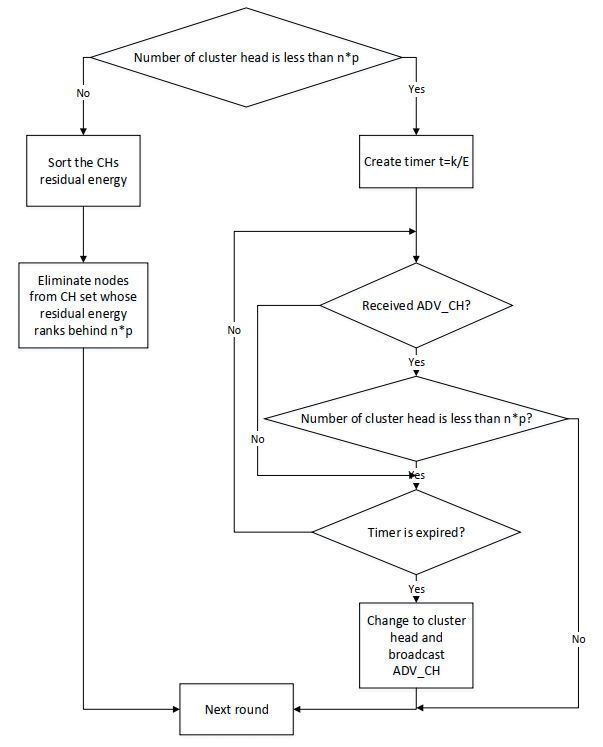
\includegraphics[width=0.8\linewidth]{1st.jpg}
		\caption{Flowchart of the second cluster head algorithm}
		\label{fig1}
	\end{figure}\\
	
	
	
	\subsection{Course}
	Finished the chapter 1 of Structuring Machine Learning Projects, Coursera, https://www.deeplearning.ai/deep-learning-specialization/
	
	\section{Objectives for the Next 2 Weeks}
	\subsection{Reading} `													
	By reading the papers, it is found that the most important parts of LEACH and improved LEACH protocols are the selection of cluster heads and the formation of the clusters. Some papers have studied to solve above problems by Kmeans. For the next two weeks, I will continue reading papers that use Kmeans in LEACH and try to propose an improved Kmeans LEACH protocol. 
	
	\section{Advisor's Comments}
	
	\bibliographystyle{IEEEtran}
	\bibliography{janbib}
	
\end{document}